\subsection{Informal Modeling}
This section is dedicated to the Informal Modeling phase description. The Section is divided in Schema and Data level in order to report the details of the elements involved in the generation of the schema, as well as the description of the datasets evolution in this phase. Moreover a specif section, one for each level, reports the difference between the elements defined in this phase and the definitions in the previous phase, analyzing in this way the variance in the different phases. 

\subsubsection{Schema level}
The schema level in this phase report the first informal definition of the ETypes and of the EER model constructed using them. 

\paragraph{ETypes and EER Model definition}\mbox{}\\
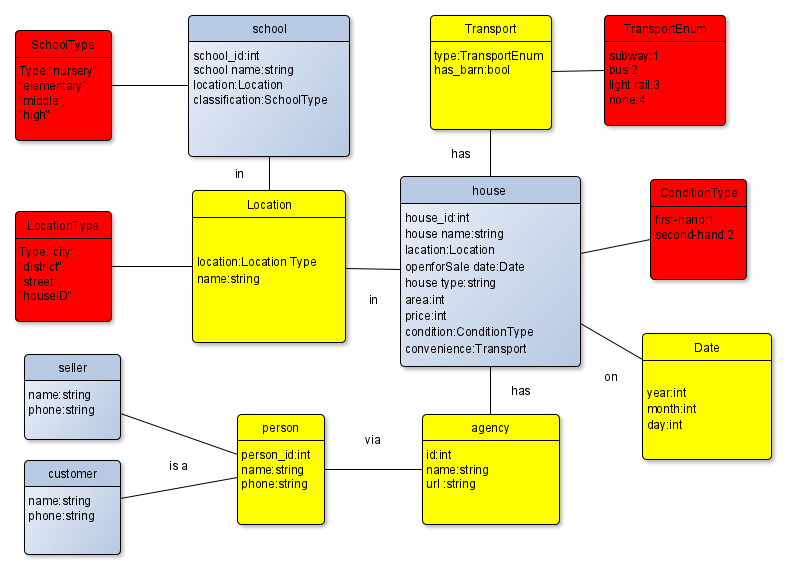
\includegraphics[width=18cm]{student codebook/sections/EER2.png}
    \caption{EER model for buy-a-house project}

To fulfill the requirement of buying a house, we built the EER model diagram above.
Among them, we use houses, sellers, buyers and schools as the core entities, because we will focus on completing the process of buying houses and dealing with the housing demand of the school district.As the most basic information of the event, the housing information should be as comprehensive as possible, so we collected the information including name, location, open-for-sale time, area, house type, price, convenience and so on.In addition, we collected the data of schools in Changchun, including school name, location and school type.We also enumerated which agent to provide the corresponding house information.

\paragraph{Variance respect CQs definition}\mbox{}\\
During the Inception phase, we discussed and developed a series of house-buying scenarios that resulted in several CQ definitions.However, after building the EER map to account for the actual situation and considering the possibility of data acquisition, our EER model may not satisfy some queries very well.For example,the definition of suburban and urban areas from metadata is not clear enough,which make it difficult to query suburban and urban homes.

\subsubsection{Data level}
The data level section in this phase reports the evolution of the datasets collected previously, reporting the metadata information for each new data, or new version of data, obtained.

\paragraph{Datasets management process}\mbox{}\\
In the formal process we got the price information about the houses and stored it in the first dataset. However, the price information in the first dataset have different kinds of forms. Some are the avarage price of the house and some are the lowest price of the house. So it's hard to get a uniform format of the result when querying the result. In this case we used the price information of the 3rd dataset which is all about the average price and replaced the origin one. And since the information of price is stored in the first dataset. We delete that in the 3rd one.And due to the format of the website we used, it's possible to get data without the property of house type and got a wrong data instead. And we found it's because they were office building so we delete the original wrong content and changed its type to office building.

\paragraph{Datasets metadata documentation}\mbox{}\\
Since in the process of cleaning datasets we only changed several value of their attributes, the datasets metadata is same as the one we given in the 2.2.4. And the concrete changes in attributes we have listed in the previous part 2.3.2.1.
\paragraph{Variance respect Inception datasets}\mbox{}\\
Since the features in the dataset are almost all literal quantities, it is difficult to use a quantitative criterion to measure the variance, so the variance-related issues are not elaborated much in this section.

\subsubsection{Informal Modeling Evaluation}
This project measures the reliability of the informal model in terms of the accuracy of the query results, i.e., the query results should not conflict with the features in the dataset. Since query requirements are diverse and the query results may exceed human common sense, reliability should be used as the evaluation index of the informal model, and too many subjective factors should not be added.